\chapter{Processo de Desenvolvimento de Jogos Eletrônicos Com Monitoramento de Dados de Saúde}\label{chap:processo_desenvolvimento}

Para a elaboração deste processo foi realizada uma revisão da literatura sobre processos de desenvolvimento de jogos tradicionais ~\cite{keith2010agile,moore2011basics,rucker2003software,kanode2009}, com o objetivo de identificar necessidades inerentes ao desenvolvimento de jogos voltados para saúde como pode ser visto em ~\cite{Suhonen_2010,herber2011,bartolome11,sinclair07,Hardy2011,kato12}. Este capítulo define um processo de desenvolvimento de jogos para entretenimento que permita o monitoramento de dados de saúde de modo não invasivo. 

%Para a elaboração desse processo foram utilizados estudos empíricos através de técnicas de pesquisa qualitativa com o uso de entrevista semi-estruturada \cite{FLI04} e observação participativa em um estudo de caso \cite{Yin05}. O resultado dessas avaliações estã descritos na \secref{section:analise_entrevista_semi_estruturada}. Como resultado dessa análise foram extraídos requisitos (\secref{section:requisitos_entrevista} e \secref{section:requisitos_estudo_caso}) que definiram algumas características e problemas de ambientes distribuídos de desenvolvimento, os quais requerem maior atenção em relação ao desenvolvimento presencial, como: uso de ferramentas colaborativas, meios de comunicação e coordenação das equipes distribuídas. 
O processo proposto, pode ser customizado posteriormente em outros contextos, desde quea equipe de desenvolvimento faça uma análise do processo e o instancie de acordo com suas necessidades.

A modelagem deste processo utiliza a semântica do meta-modelo \ac{spem} na Versão 2.0 \cite{spem08}, que permite modelar: métodos, atividades de processos de software através da notação gráfica UML. 

\section{Visão Geral}
O processo proposto chamado de \textit{GAHME Process}, tem como objetivo principal guiar o desenvolvimento de jogos eletrônicos com o objetivo monitorar dados de saúde (\textit{GAHME}). Desta maneira, pode-se dizer que a principal contribuição deste processo é fornecer um conjunto coerente de atividades e artefatos direcionados para o desenvolvimento de um \textit{GAHME}, mas que mantém a generalidade de um processo de desenvolvimento de \textit{software}, e pode ser aplicado no contexto de desenvolvimento de jogos.
%
%\begin{figure}
 %\centering
 %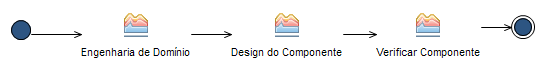
\includegraphics[scale=0.8]{./img/visaogeral.png}
 %% matrixargseg.png: 296x162 pixel, 100dpi, 7.52x4.11 cm, bb=0 0 213 117
 %%\caption{Estágio desenvolvimento de jogos ~\cite{fullerton2008game}}
%\caption{Visão Geral \textit{GAHME Process}}
%%  \caption{Estágio desenvolvimento de jogos}
 %\label{fig:visaogeral}
%\end{figure}
%
Atualmente, o \textit{GAHME Process} contempla duas fases distintas com responsabilidades definidas:
	%\begin{enumerate}
		%\item \textbf{Viabilidade:} A primeira fase deverá ser realizado um estudo sobre o público alvo, sintomas a serem monitorados, técnicas e tecnologias que permitam o monitoramento e a viabilidade de realizar o monitoramento dos dados de saúde por intermédio dos jogos eletrônicos.		
		%\item \textbf{Desenvolvimento:} A segunda fase utilizará os artefatos de software produzidos durante a primeira fase do processo para desenvolver um jogo eletrônico que permita realizar o monitoramento dos dados de saúde. No final da fase deverá ser realizada uma pesquisa com o público alvo do sistema para comprovar a eficácia do monitoramento.
	%\end{enumerate}
	
	\begin{enumerate}
	\item \textbf{Conceito:} responsável em definir o público alvo do jogo, identificar a população beneficiada, e avaliar o impacto do desenvolvimento do jogo. É de responsabilidade desta fase avaliar os sintomas monitoráveis bem como a existência de sensores capacitados. O término da fase será um estudo da viabilidade do monitoramento dos sintomas por meio dos jogos eletrônicos.
	\item \textbf{Pré-Produção:} definir as tecnologias utilizadas para o desenvolvimento do jogo, e testar a aquisição do sinal pelos sensores utilizando um protótipo desenvolvido. 
	Na Pré-Produção são elaborados cenários de jogos que permitam o monitoramento de dados, depois faz-se testes com os protótipos para a elaborar um artefato que define as ações monitoráveis dos jogadores (\textit{GAHME Action Design} Seção~\ref{subsec:game_actions_guide}).
\end{enumerate}

\section{Papéis e Responsabilidades}
A descrição dos papéis presentes no processo é importante para um melhor entendimento das atividades realizadas no processo. Nesta seção serão descritos os papéis previstos assim como suas principais habilidades e atribuições.


\subsection{\textit{Game Designer}}\label{subsec:game_designer}
O projeto de um jogo eletrônico é uma atividade multidisciplinar e requer a contribuição de diversos perfis e habilidades. O \textit{Game Designer} deve trabalhar em colaboração com todos os membros da equipe de desenvolvimento como Engenheiro de Software, \textit{Art Designer} e saber dos anseios do jogador ~\cite{schell2008art}. Um bom \textit{Game Designer} está disposto a escutar as diferentes opiniões e sugestões, para selecionar aquelas que melhorem a experiência do jogo ~\cite{moore2011basics}. Esse papel é responsável pela concepção, passando por atividades de: análise, melhorar o \textit{game design} e verificar o produto final.

\subsubsection{Habilidades}
Para desempenhar este papel é necessário que o integrante tenha as seguintes habilidades:
  \begin{itemize}
	  \item Entender dos anseios e ponto de vista do jogador em relação ao jogo ~\cite{schell2008art};
		\item compreender as ações monitoráveis do jogador definidos no \textit{GAHME Action Design} (Seção \ref{subsec:game_actions_guide});
		\item conceber o jogo o que confere narrativa, regras e objetivos~\cite{schell2008art,moore2011basics,bethke2003game}.
  \end{itemize}

\subsubsection{Abordagens de Atribuição}
O \textit{Game Designer} precisa conhecer as capacidades técnicas da equipe e das ações que monitoráveis do jogo, documentadas no \textit{GAHME Action Design}.

\subsection{\textit{Game Health Designer}}
O \textit{Game Health Designer} tem um papel bem parecido com o do \textit{Game Designer} (Seção \ref{subsec:game_designer}), mas com a responsabilidade de trabalhar em colaboração com o Profissional de Saúde e com o Engenheiro de Software para verificar a viabilidade do jogo. 

O \textit{Game Health Designer} elabora o \textit{GAHME Action Design} (Seção \ref{subsec:game_actions_guide}) que é o artefato que faz o mapeamento das ações monitoráveis e sua relação com os dados de saúde. 

\subsubsection{Habilidades}
Para desempenhar este papel é preciso:
  \begin{itemize}
	  \item Compreender as diretrizes médicas (Seção \ref{subsec:diretrizes_medicas});
		\item extrair sintomas monitoráveis com o auxílio do Profissional de Saúde;
		\item analisar as possibilidades de monitoramento por meio dos sensores disponíveis com o auxílio do Engenheiro de Software;
		\item verificar a viabilidade do monitoramento dos dados de saúde por meio de um jogo eletrônico;
		\item conceber um artefato de \textit{GAHME Action Design} que auxilie na concepção de um jogo.
  \end{itemize}

\subsubsection{Abordagens de Atribuição}
O \textit{Game Health Designer} deve ter conhecimento tanto da área de saúde quanto das tecnologias utilizadas no desenvolvimento dos jogos.

\subsection{Engenheiro de \textit{Software}}\label{subsec:engenheiro_software}
Esse papel é responsável por desenvolver o sistema. Os engenheiros de software utilizam como entrada o \textit{GAME Design} e o \textit{GAHME Action Guideline} gerado pelos \text{Designers}. É de extrema importância que esse perfil compreenda o \textit{GAME Design} para que o jogo desenvolvido esteja de acordo com sua especificação.

\subsubsection{Habilidades}
Para desempenhar este papel é preciso:

\begin{itemize}
    \item Definir e criar soluções técnicas através das tecnologias utilizadas no projeto.
		\item Comunicar e repassar a arquitetura da aplicação para os demais integrantes.
\end{itemize}

\subsubsection{Abordagens de Atribuição}
O perfil do engenheiro de software é mais técnico. Esse profissional deve dominar a tecnologia de desenvolvimento de jogos utilizada além de compreender da capacidade dos sensores utilizados no projeto.

\subsection{Profissional de Saúde}\label{subsec:profissional_saude}
O profissional de saúde representa o grupo interessado em receber os dados dos usuários, os quais serão monitorados. O compreendimento das necessidades e interesses desse profissional são elementos chave para o desenvolvimento de uma solução efetiva.

\subsubsection{Habilidades}
O papel de Profissional de Saúde detém o expertise da doença e dos sintomas monitorados.

\subsubsection{Abordagens de Atribuição}
O Profissional de Saúde, presente no processo de desenvolvimento, deve fornecer o conhecimento sobre os sintomas referentes a sua especialidade de formação. Auxiliando na compreensão dos sintomas e das ações dos usuários, que devem possibilitar o monitoramento.

Algumas doenças são acompanhadas por diferentes Profissionais de Saúde, sejam médicos e fisioterapeutas ou até mesmo médicos com diferentes especializações. Nestes casos, é necessário a participação dos diferente perfis de profissionais de saúde para que sejam colhidas informações com mais detalhes e possa envolver a opinião dos diferentes profissionais.




\section{Fase: Conceito}\label{sec:conceito}
A fase de Conceito tem como papéis principais para sua execução o \textit{Game Health Designer} e o \textit{Profissional de Saúde}. Estes perfis fazem a análise da viabilidade do monitoramento. Terminada essa atividade, o \textit{Game Designer} elabora cenários de jogos que permitem o monitoramento. Baseado nos cenários, o Engenheiro de \textit{Software} implementa protótipos de jogos para testar a abordagem. 

Por se tratar de um jogo voltado para o monitoramento da saúde, as diretrizes médicas possibilitará o suporte científico para interpretação dos dados. Podem ser analisados e reproduzidos os trabalhos científicos da área, para verificar a viabilidade de um jogo a ser desenvolvido.

\begin{figure}[!htb]
 \centering
 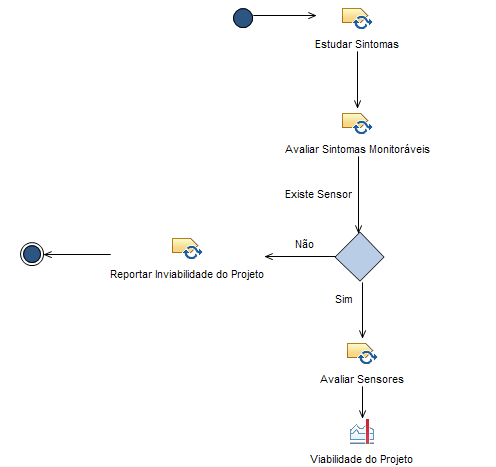
\includegraphics[scale=0.8]{./img/gahme-fase-conceito.png}
 % matrixargseg.png: 296x162 pixel, 100dpi, 7.52x4.11 cm, bb=0 0 213 117
 %\caption{Estágio desenvolvimento de jogos ~\cite{fullerton2008game}}
\caption{Fase de Conceito do \textit{GAHME Process}}
%  \caption{Estágio desenvolvimento de jogos}
 \label{fig:faseviabilidade}
\end{figure}


\subsection{Atividade: Identificar Público Alvo}
O \textit{Game Health Designer} define o perfil do jogador, essa é uma questão importante, pois define o público alvo do jogo. Isso ocasiona em avaliar a faixa etária a que se destina o jogo, pois jogos desenvolvidos para um público infantil tem um perfil bastante diferente dos voltados para adultos ~\cite{brathwaite2009challenges}. Por isso, o público alvo impacta diretamente na elaboração do \textit{Game Design} do projeto, pois o perfil do usuário pode necessitar de ambientes mais lúdicos em caso de crianças ~\cite{yannakakis06}, ou uma maior preocupação com situações de risco para caso o jogo seja direcionado para os idosos ~\cite{brox11,arntzen2011}.


\subsubsection{Papéis Responsáveis}
\begin{itemize}
	\item \textit{Game Health Designer};
	\item Profissional de Saúde.
\end{itemize}

\subsubsection{Passos para Execução da Atividade}
\begin{itemize}
	\item Avaliar faixa etária;
	\item avaliar necessidade de monitoramento;
	\item avaliar sintomas a serem monitorados.
\end{itemize}

\subsubsection{Artefatos de Entrada}
\begin{itemize}
	\item Diretrizes Médicas.
\end{itemize}

\subsubsection{Artefatos de Saída}
\begin{itemize}
	\item Seção de Análise de Impacto do documento de \textit{GAHME Design}.
\end{itemize}


\subsection{Atividade: Estudar Sintomas}
O objetivo principal dessa atividade é identificar sintomas monitoráveis usando as Diretrizes Médicas como base científica para a execução desta atividade e a opinião do Profissional de Saúde para melhor entendimento do sintoma e das práticas exercidas para a sua identificação. O \textit{Game Health Designer} faz um mapeamento dos sintomas e possíveis valores que identifiquem a sua ocorrência. 

O objetivo dessa atividade é identificar os sintomas monitoráveis sem levar em consideração a existência ou as especificações técnicas dos sensores que possibilite o monitoramento dos dados. 

\subsubsection{Papéis Responsáveis}
\begin{itemize}
	\item \textit{Game Health Designer};
	\item Profissional de Saúde.
\end{itemize}

\subsubsection{Passos para Execução da Atividade}
\begin{itemize}
	\item Identificar sintomas;
	\item avaliar necessidade de monitoramento dos sintomas;
	\item Descrever sintomas passíveis de monitoramento.
	%\item Especificar valores que identifiquem os sintomas;	
\end{itemize}

\subsubsection{Artefatos de Entrada}
\begin{itemize}
	\item Diretrizes Médicas.
\end{itemize}

\subsubsection{Artefatos de Saída}
\begin{itemize}
	\item Seção de Sintomas Passíveis de Monitoramento do documento de \textit{GAHME Design}.
\end{itemize}

\subsection{Avaliar Sintomas Monitoráveis}
Baseado na Seção de Sintomas Passíveis de Monitoramento do documento de \textit{GAHME Design} e na Especificação dos Sensores existentes o \textit{Game Health Designer} irá identificar e descrever quais são os sintomas monitoráveis. Para a elaboração deste artefato faz-se necessária a colaboração do Engenheiro de \textit{Software} por ter habilidades em tecnologia e este ser mais habilitado a compreender as especificação do sensor. O Profissional de Saúde tem papel auxiliar para esclarecer dúvidas sobre os sintomas e como o monitoramento deve ser efetuado.

O \textit{Game Health Designer} participa das discussões de saúde e tecnológicas, pois ele irá conceber quais serão as ações executadas pelo jogador, logo ele necessita entender tanto das limitações técnicas dos sensores quanto dos movimentos que o jogador efetua. 

%Para a execução desta atividade o \textit{Game Health Designer} deverá fazer uso do Documento de Diretrizes Médicas (Seção \ref{subsec:diretrizes_medicas}) para identificar a necessidade de monitoramento dos sintomas, juntamente com o Profissional de Saúde, deverão selecionar sintomas que identifique problemas de saúde e que sejam mensuráveis por intermédio de sensores. Durante a execução desta atividade também deve ser coletado as informações a respeito da importância, impactos e benefícios ao tratamento de saúde o público alvo terá ao ter esses sintomas monitorados.

\subsubsection{Papéis Responsáveis}
\begin{itemize}
	\item \textit{Game Health Designer};
	\item Engenheiro de \textit{Software};
	\item Profissional de Saúde.
\end{itemize}

\subsubsection{Passos para Execução da Atividade}
\begin{itemize}
	\item Analisar os sintomas monitoráveis;
	\item coletar sensores que possibilitem o monitoramento;
	\item estudar os principais sensores;
	\item mapear sintomas e sensores que possibilitem o monitoramento dos dados.
\end{itemize}

\subsubsection{Artefatos de Entrada}
\begin{itemize}
	\item Seção de Sintomas Monitoráveis do documento de \textit{GAHME Design}
\end{itemize}

\subsubsection{Artefatos de Saída}
\begin{itemize}
	\item Seção de Sintomas Monitorados do documento de \textit{GAHME Design}
\end{itemize}

%\subsection{Criar Arcabouço de \textit{Software} Para Captura de Dados}
%%Caso a equipe de desenvolvimento não tenha conhecimento ou experiência sobre uma \textit{engine} de jogos que atendam as necessidades do jogo para monitoramento de dados de saúde, 
%Essa atividade consiste em desenvolver um Arcabouço de \textit{Software}, que consiga adquirir dados dos sintomas passíveis de monitoramento conforme o \textit{GAHME Design}.
%
%O Engenheiro de \textit{Software} irá analisar as \textit{engine} de jogos existentes e os mecanismos que permitam integrar essa \textit{engine} com os sensores utilizados no jogo. Sensores como o acelerômetro do celular já possuem suporte nativo dentro das \textit{engine} de jogos para esses dispositivos ~\cite{unity3d}. Outros sensores como o MS-Kinnect ~\cite{kinnect2013} que é uma câmera que permite adquirir os movimentos do corpo, necessitam da instalação de \text{Device Drivers} e \textit{Componentes} de software a serem instalados dentro da \textit{engine} ~\cite{zigfu} para permitir a integração. Como referência a essa atividade podemos citar o trabalho de mestrado de Santos Jr.~\cite{antonio2013} que criou um arcabouço de software para monitoramento de dados de saúde com as tecnologias de acelerômetro presentes em celulares Android e do MS-Kinnect~\cite{kinnect2013}. 
%
%Nessa atividade também o Engenheiro de \textit{Software} pode identificar barreiras tecnológicas que inviabilizem o monitoramento dos sintomas. Nesse caso ele deve reportar a inviabilidade do projeto e terminar o ciclo de desenvolvimento. 
%
%\subsubsection{Papéis Responsáveis}
%\begin{itemize}
	%\item Engenheiro de \textit{Software};
%\end{itemize}
%
%\subsubsection{Passos para Execução da Atividade}
%\begin{itemize}
	%\item Analisar os sintomas passíveis de monitoramento;
	%\item coletar sensores que possibilitem o monitoramento dos sintomas;
	%\item estudar os principais sensores coletados;
	%\item mapear sintomas e sensores que possibilitem o monitoramento dos dados.
%\end{itemize}
%
%\subsubsection{Artefatos de Entrada}
%\begin{itemize}
	%\item Seção de Sintomas Passíveis de Monitoramento do documento de \textit{GAHME Design}
%\end{itemize}
%
%\subsubsection{Artefatos de Saída}
%\begin{itemize}
	%\item Arcabouço de \textit{Software} Para Captura de Dados..
%\end{itemize}

\subsection{Reportar Inviabilidade do Projeto}
A inviabilidade do projeto pode ter diferentes fatores, essa atividade ficará a cargo do Engenheiro de \textit{Software}, para a tomada de decisão, ele faz a captura dos sinais e verifica se o sensor tem a precisão necessária para identificar os sintomas. Caso o sensor ou as ações não sejam monitoráveis o Engenheiro de \textit{Software} elabora um documento justificando a inviabilidade do projeto.
%Existem casos que os sensores são capazes de adquirir os dados dos sintomas mas as ações dos usuários não podem ser utilizadas em um jogo eletrônico. Como por exemplo o sintoma de Tremor da ~\ac{dp} que é de repouso ~\cite{patel_monitoring_2009}. A \textit{priori}, não existe barreira tecnológica para identificar o sintoma de tremor usando os acelerômetros de um aparelho de celular e logicamente identificar o sintoma parkinsoniano. Mas, pacientes com essa patologia ao interagir com o dispositivo usando a mão, entram num estado ativo do membro cessando assim o tremor naquele momento inviabilizando o monitoramento e como consequência o projeto.

\subsubsection{Papéis Responsáveis}
\begin{itemize}
	\item Engenheiro de \textit{Software}.
\end{itemize}

\subsubsection{Papéis Auxiliares}
\begin{itemize}
	\item Profissional de Saúde.
\end{itemize}

\subsubsection{Passos para Execução da Atividade}
\begin{itemize}
	\item Analisar precisão dos sensores e comparar com os sintomas monitoráveis;
	\item explicar motivos que tornaram o monitoramento inviável.
\end{itemize}

\subsubsection{Artefatos de Entrada}
\begin{itemize}
	\item Seção de Sintomas Monitorados do documento de \textit{GAHME Design};
\end{itemize}

\subsubsection{Artefatos de Saída}
\begin{itemize}
	\item Seção de Inviabilidade de Monitoramento do documento de \textit{GAHME Design}
\end{itemize}



\section{Fase: Pré-Produção}
Os jogos para saúde precisam passar por pesquisa entre seres humanos e testado com grupo de controle para verificar sua eficácia~\cite{kato12}. Na pré-produção (Figura~\ref{fig:fasedesenvolvimento}), deve ser desenvolvido um protótipo do jogo para verificar sua viabilidade. Logo, se o protótipo desenvolvido for testado com seres humanos e os dados forem testados com uma boa eficácia finaliza-se a pré-produção. De posse dos artefatos deste processo, pode-se executar o ciclo de desenvolvimento de um jogo tradicional como definido em ~\cite{fullerton2008game}.

A fase de Pré-Produção tem como papéis principais para sua execução o \textit{Game Designer} e o Engenheiro de \textit{Software} e como resultado final a comprovação da eficácia do protótipo do jogo em relação ao monitoramento dos dados de saúde. 
\begin{figure}[!HTB]
 \centering
 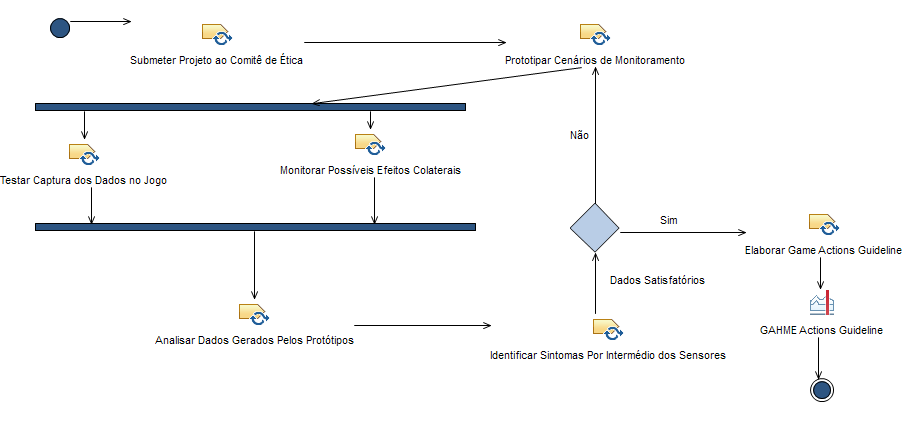
\includegraphics[scale=0.6]{./img/gahme-fase-pre-producao.png}
 % matrixargseg.png: 296x162 pixel, 100dpi, 7.52x4.11 cm, bb=0 0 213 117
 %\caption{Estágio desenvolvimento de jogos ~\cite{fullerton2008game}}
\caption{Fase de Pré-Produção do \textit{GAHME Process}}
%  \caption{Estágio desenvolvimento de jogos}
 \label{fig:fasedesenvolvimento}
\end{figure}
\FloatBarrier



%Nos últimos anos houve um crescimento de jogos voltados para saúde, contudo muito desses jogos não foram validados efetivamente ou foi realizado um estudo para verificar os seus resultados ~\cite{kato12}. Os estudos realizados por muitos desses jogos foram mal projetados e suas conclusões não podem se consideradas válidas ou eficazes. Por esse motivo Kato ~\cite{kato12} sugeriu diretrizes para a realização de estudos de eficácia para ser aplicados em jogos para saúde. 
%Como a iteração de "Verificação" é responsável por avaliar a eficácia do monitoramento dos dados de saúde a partir do jogo desenvolvido, as sugestões definidas por Kato ~\cite{kato12} estarão presentes no decorrer da iteração.






%

%
%\begin{enumerate}
	%\item \textbf{Desenvolvimento:} A iteração de implementação será bem semelhante a uma fase de produção de um jogo tradicional ~\cite{fullerton2008game}, tendo como produto final da fase o jogo desenvolvido. Contudo, o \textit{Game Design} deverá levar em consideração as ações do jogador que permitem monitoramento (\textit{GAHME Actions Guideline}). No término desta fase, o jogo deverá ser testado com o objetivo de identificar se os mecanismos de captura de dados de saúde do jogo foram desenvolvidos corretamente.
	%\item \textbf{Verificação:} 	O desenvolvimento de um jogo por si só é uma tarefa multidisciplinar ~\cite{fullerton2008game} e esta quando aplicada num contexto de saúde necessita de mecanismos para verificar a eficácia da abordagem adotada ~\cite{kato12}. Nessa fase, a proposta do jogo deverá ser submetida para a avaliação do conselho de ética médica, para que possa ser testado com seres humanos e verificar se os sintomas monitorados foram corretamente identificados.
%\end{enumerate}

\subsection{Submeter Projeto ao Comitê de Ética}
O objetivo dessa atividade é submeter o protótipo do jogo às normas regulamentadoras previstas para a pesquisa envolvendo seres humanos segundo a Resolução 196/96 ~\cite{conselho2000normas}. Segundo o Conselho Nacional de Saúde ~\cite{conep2002}, o ~\ac{cep} é um colegiado interdisciplinar e independente,  que deve existir nas instituições que realizam pesquisas envolvendo seres humanos no Brasil, criado para defender os interesses dos sujeitos da pesquisa em sua integridade e dignidade e para contribuir no desenvolvimento da pesquisa dentro de padrões éticos (Normas e Diretrizes Regulamentadoras da Pesquisa Envolvendo Seres Humanos - Res. CNS 196/96 ~\cite{conselho2000normas}). 

O \ac{cep} é responsável pela avaliação e acompanhamento dos aspectos éticos de todas as pesquisas envolvendo seres humanos. Este papel está bem estabelecido nas diversas diretrizes éticas internacionais (Declaração de Helsinque, Diretrizes Internacionais para as Pesquisas Biomédicas envolvendo Seres Humanos – CIOMS) e Brasileiras (Res. CNS 196/96 e complementares~\cite{conselho2000normas}), diretrizes estas que ressaltam a necessidade de revisão ética e científica das pesquisas envolvendo seres humanos, visando a salvaguardar a dignidade, os direitos, a segurança e o bem-estar do sujeito da pesquisa ~\cite{conep2002}.
%
%Nessa atividade deve ser elaborado um Protocolo de Pesquisa, contemplando a descrição da pesquisa, estabelecer critérios de inclusão e exclusão dos sujeitos da pesquisa, a qualificação dos pesquisadores e todas instâncias responsáveis pelo projeto. Estão presentes no projeto Instituições de pesquisa, legitimamente constituída e habilitada que permita realizar as investigações científicas. 

Os pesquisadores elegem os riscos da pesquisa, principalmente danos físicos, psíquicos, moral, intelectual, cultural do ser humano em qualquer fase de uma pesquisa dela decorrente ~\cite{conselho2000normas}. Sendo necessária a anuência do sujeito da pesquisa ou de um representante por intermédio do Consentimento livre e esclarecido, onde será explicado a natureza da pesquisa, seus objetivos, métodos, benefícios previstos, potenciais riscos e o incômodo que esta possa acarretar, formulada em um termo de consentimento, autorizando sua participação voluntária na pesquisa ~\cite{conselho2000normas}. Caso o sujeito da pesquisa se enquadre nos critérios estabelecidos para interromper a pesquisa, essa deverá ser finalizada assegurando a integridade do mesmo. Como o Profissional de Saúde possui em sua formação a natureza da pesquisa além de conhecer os métodos que serão aplicados durante a pesquisa ele possui o perfil mais habilitado para desempenhar essa atividade.


Atualmente no Brasil para poder testar o jogo com monitoramento de dados de saúde junto a pacientes, e consequentemente testar sua eficácia, é necessário passar por esse processo e obter a aprovação de um \ac{cep}. Este é um processo demorado e pode impactar a entrega final.

\subsubsection{Papéis Responsáveis}
\begin{itemize}
	\item Profissional de Saúde.
\end{itemize}

\subsubsection{Passos para Execução da Atividade}
\begin{itemize}
	\item Analisar os sintomas a serem monitorados;
	\item Identificar objetivo da pesquisa;
	\item Identificar potenciais riscos e estabelecer critérios para interromper a pesquisa;
	\item Identificar benefícios previstos.
\end{itemize}

\subsubsection{Artefatos de Entrada}
\begin{itemize}
	\item Diretrizes Médicas;
	\item Seção de Sintomas Monitorados do documento de \textit{GAHME Design}.
\end{itemize}

\subsubsection{Artefatos de Saída}
\begin{itemize}
	\item Projeto Submetido ao Comitê de Ética Médica;
	\item Termo de Consentimento Livre e Esclarecido.
\end{itemize}

%\subsection{Identificar Sintomas Por Intermédio dos Sensores}
%Baseado nos

 

%\subsection{Monitorar Possíveis Efeitos Colaterais}
%Durante a execução da pesquisa possíveis efeitos colaterais devem ser monitorados como: risco de queda, fadiga, tendinite. 
%As avaliações de jogos para a saúde devem tentar controlar o uso de seu jogo para efeitos colaterais negativos, outro possível efeitos colateral negativo dos jogos é a ocorrência de convulsões, devido à fotossensibilidade.








\subsection{Verificar Eficácia do Jogo}
A eficácia do jogo será verificada através de um estudo analítico de caso-controle ~\cite{menezes2001epidemiologia}, dentro de um ambiente aprovado pelo \ac{cep} que permitirá recrutar sujeitos de pesquisa. Uns sujeitos deverão apresentar os sintomas a serem monitorados e outros não terão tais sintomas. Os dados serão coletados e ao final deverá ser verificado se os sintomas foram corretamente identificados.

Kato ~\cite{kato12} defende que para essa verificação é necessário obter um número adequado de participantes para conseguir avaliar o impacto do jogo. Contudo, determinados sintomas possuem poucos sujeitos de pesquisa disponíveis reduzindo a abrangência da pesquisa.

%Em uma revisão sistemática sobre a eficácia dos jogos existes e que promovem a atividade física para adolescentes ~\cite{foley-active-game2010}, segundo a revisão a abordagem de jogos se mostrou eficaz ao motivar a execução de atividade física dos usuários. Os jogos estudaram envolveram tanto os membros superiores quanto inferiores do corpo melhorando a atividade de forma prazerosa e com qualidade inclusive em grupos de deficiência e de alto risco.

%Verificar essa referencia ~\cite{Primack2012630}

%\subsection{Atividade: Publicar Resultados}


\subsection{Atividade: Elaborar \textit{GAHME Design}}
De posse dos movimentos e da captura dos dados descritos no \textit{Game Action Guideline}. ´É elaborado um \textit{game design} inclui os movimentos no contexto do jogo eletrônico ~\cite{sweetser2005-gameflow}, este jogo possui mecanismos de monitoramento dos dados de saúde embutidos. Para a execução desta atividade, leva-se em consideração um processo iterativo, que precisa é: protipar, testar e refinar continuamente até concluir~\cite{brathwaite2009challenges}.



%\section{Iteração: Prototipação}
%O objetivo desta iteração é desenvolver um protótipo que permita capturar dados de saúde e ao término desta iteração deverá ser elaborado o \textit{GAHME Actions Guideline} (Seção \ref{subsec:game_actions_guide}) que conterá as ações executadas pelo jogador que possam ser monitoráveis e que venham a ser utilizadas pelo \textit{Game Designer} durante a fase de Desenvolvimento. 
%
%Alinhar a jogabilidade e a possibilidade de monitoramento frequente dos dados de saúde não é uma tarefa trivial. Pois deve ser levado em consideração o uso dos dispositivos e pensar na execução de movimentos ou ações que permitam esse monitoramento. Para propor um jogo com monitoramento de dados de saúde deve ser realizado um estudo sobre quais os movimentos e ações que o usuário deve executar. De posse dessas ações, deve ser desenvolvidos protótipos que permitam testar a execução dessas atividades e capturar os dados com o objetivo de estudar mecanismos que permitam identificar esses sintomas conforme os trabalhos já existentes e que possuem tal propósito ~\cite{Ballegaard:2008:HEL:1357054.1357336,albanese2012,bachlin_wearable_2010,visionbased2009,patel_monitoring_2009}. 
%
%\begin{figure}
 %\centering
 %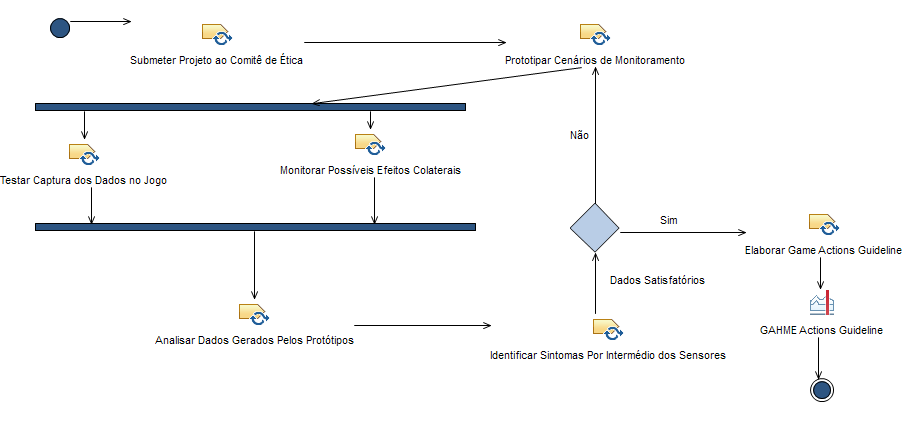
\includegraphics[scale=0.55]{./img/gahme-fase-pre-producao.png}
 %% matrixargseg.png: 296x162 pixel, 100dpi, 7.52x4.11 cm, bb=0 0 213 117
 %%\caption{Estágio desenvolvimento de jogos ~\cite{fullerton2008game}}
%\caption{Iteração: Prototipação do \textit{GAHME Process}}
%%  \caption{Estágio desenvolvimento de jogos}
 %\label{fig:prototipaccao}
%\end{figure}


%Os movimentos não podem ser repetitivos pois, levaria o usuário jogar por um curto período e como consequência abandonaria o monitoramento ~\cite{Suhonen:2008:SFE:1457199.1457204}. 



 

%\subsection{Engenheiro de Software}
%Esse papel é responsável por desenvolver o sistema. Os engenheiros de
%software devem utilizar como entrada o \useacronym{DER} gerado pelos engenheiros de requisitos. É
%de extrema importância que os engenheiros de software entendam o
%\useacronym{DER} para que o produto desenvolvido esteja de acordo com sua
%especificação.
%
%\textbf{Habilidades}
%
%Para desempenhar este papel é necessário que o integrante tenha o
%perfil com as  seguintes habilidades:
%
%\begin{compactenum}
    %\item Definir e criar soluções técnicas através das tecnologias utilizadas no projeto.
    %\item Identificar e construir casos de teste que venham cobrir o
%comportamento requerido pelos componentes do sistema.
    %\item Comunicar e repassar a arquitetura da aplicação para os
    %demais integrantes.
%\end{compactenum}
%
%\textbf{Abordagens de Atribuição}
%Mesmo em equipes pequenas, os indivíduos devem trabalhar em grupo no
%desenvolvimento de soluções técnicas.
%
%Cada integrante pode executar tarefas especificas de acordo com suas
%habilidades, porém é desejável que as demais tecnologias utilizadas
%no projeto sejam do conhecimento de todos, para que haja uma maior
%troca de auxilio técnico entre os integrantes.




\section{Artefatos}

%Os documentos para o desenvolvimento de jogos tem dois propósitos principais: histórico do projeto e comunicação ~\cite{schell2008art}. O desenvolvimento de um jogo requer a tomada de decisões a todo o momento, que definem o funcionamento do jogo. Contudo, existe uma grande probabilidade de que os envolvidos do projeto não se recordem dos motivos que as decisões foram tomadas. Se a equipe de desenvolvimento tiver o hábito de armazenar todas as tomadas de decisões e documentá-las nos artefatos utilizados no desenvolvimento do software então não será necessário rediscutir as decisões já tomadas ~\cite{schell2008art}.
Os artefatos de software servem como documentos de entrada e saída da execução de atividades dentro do próprio processo ~\cite{sommerville2011}.

\subsection{Diretrizes Médicas}\label{subsec:diretrizes_medicas}
O principal propósito da atividade médica é o cuidado com o paciente, e isso traz enormes desafios de forma coletiva ou individual. Com o intuito de auxiliar na tomada de decisões, a comunidade médica mundial tem elaborado e divulgado um extenso número de informações ~\cite{nhs2013,neozeland-guide-2013}, muito mais acessíveis do que era no passado, redefinindo o universo do conhecimento médico, tornando-o livre e acessível para críticas e demais propósitos científicos ~\cite{proj-diretriz2013}.

%Neste contexto, a Associação Médica Brasileira e o Conselho Federal de Medicina, com o objetivo de auxiliar na tomada de decisão médica e, consequentemente, otimizar o cuidado aos pacientes, desencadearam um processo junto às Sociedades de Especialidade para a elaboração de Diretrizes Médicas baseadas nas evidências científicas disponíveis na atualidade ~\cite{proj-diretriz2013}.
%
%Nesse processo, formou-se uma Comissão Técnica responsável em construir as bases de sustentação das recomendações de conduta médica, utilizando os meios da ciência atual, de forma crítica e desprovida de interesse se não aquele que resulte na melhoria do tratamento do médico com o paciente. 

Partindo do princípio que o conhecimento médico atual está presente nas diretrizes médicas e que através do seu conteúdo é possível extrair informações que permitam: identificar, avaliar a presença e evolução de sintomas de doenças. 
%Nas diretrizes médicas estão descritos mecanismos de diagnósticos, prognóstico, tratamento, dosagem medicamentosa, riscos e benefícios. Além de definir questões mais relacionadas à prática clínica e descrevendo as possíveis opções para a tomada de decisão sobre o tratamento da doença .a ser monitorada como por exemplo a Doença de Parkinson que servirá como estudo de caso do presente trabalho ~\cite{protpar010}.
%evidências através dos dados sobre a doença bem como mecanismos de diagnósticos, prognóstico, tratamento, dosagem medicamentosa, riscos e benefícios. Além de definir questões mais relacionadas à prática clínica e descrevendo as possíveis opções para a tomada de decisão sobre o tratamento da doença .a ser monitorada como por exemplo a Doença de Parkinson que servirá como estudo de caso do presente trabalho ~\cite{protpar010}.
\subsubsection{Propósito}
As diretrizes médicas permitem identificar sintomas monitoráveis, bem como parâmetros relevantes a esses sintomas. Este documento é escrito pela comunidade médica e é considerado como base científica sobre o tema abordado. Para o \textit{GAHME Process} este artefato servirá de artefato de entrada para fundamentar quais sintomas serão monitorados e de que forma serão avaliados.


%\subsection{Estudos Epidemiológicos}\label{subsec:estudos_epidemiologicos}
%A Epidemiologia é a ciência que estuda ocorrência de doenças em populações humanas e seus fatores determinantes das doenças ou condições relacionadas à saúde em populações especificadas no estudo ~\cite{menezes2001epidemiologia,lima-costa-2003}. Inicialmente a epidemiologia restringia-se a estudo de epidemias de doenças transmissíveis, contudo atualmente a epidemiologia trata qualquer evento relacionado à saúde (ou doença) da população ~\cite{menezes2001epidemiologia}.
%
%%\subsubsection{Tipos de Estudos epidemiológicos}
%Os estudos epidemiológicos podem ser classificados em observacionais e experimentais, para o este trabalho serão utilizados estudos epidemiológicos observacionais descritivos têm por objetivo determinar a distribuição de doenças ou condições relacionadas à saúde, segundo o tempo, o lugar e/ou as características dos indivíduos ~\cite{lima-costa-2003}. Ou seja, responder à pergunta: quando, onde e quem adoece? Logo, as respostas dessas perguntas serão fundamentais para avaliar o impacto de possíveis tratamentos, medicamentos trabalho ou em nosso caso do desenvolvimento de um jogo que permita o monitoramento de dados de saúde.
%
%A epidemiologia descritiva pode fazer uso de dados secundários (dados pré-existentes de mortalidade e hospitalizações, por exemplo) e primários (dados coletados para o desenvolvimento do estudo) ~\cite{lima-costa-2003}. No Brasil, existem importantes bancos de dados secundários com abrangência nacional que podem ser usados para estudo epidemiológicos como: Sistema de Informações sobre Mortalidade (SIM-SUS) ~\cite{sis2013}, Pesquisa Nacional de Amostra Domiciliar (PNAD) ~\cite{pnad2008} bem como os estudos epidemiológicos realizados no Brasil e disponibilizados em Bases de estudo em saúde como Scielo ~\cite{scielo2013}.

%\subsubsection{Propósito}
%O propósito deste artefato é identificar a população beneficiada como o monitoramento dos dados de saúde por intermédio dos jogos eletrônicos.


\subsection{\textit{GAHME Action Design}}\label{subsec:game_actions_guide}
\subsubsection{Documento de Sintomas Monitoráveis}
Esse artefato é o princial artefato da fase de \textit{Concepção}, é através dele que será decidida a viabilidade do desenvolvimento do jogo nas fases seguintes do processo de desenvolvimento. Contudo, mesmo sendo um artefato elaborado na primeira fase do processo de desenvolvimento, este não será descartado nas demais fases pois deverá ser testado e refinado nas fases seguintes do processo.


\subsubsection{Cenário de Jogo}
A fase de conceito do cenário do jogo para muito autores é definida como crucial para conseguir um jogo de sucesso e atingir elementos difíceis de ser mensurados como por exemplo a diversão. O uso de protótipos nas etapas iniciais do processo de desenvolvimento permitem anteceder o comportamento do jogo e auxiliar na definição do mesmo durante a elaboração do \textit{Game Design}, pois os jogadores podem experimentar o jogo nas etapas iniciais e permite que estes teçam suas opiniões~\cite{prototipgames2007}.
 
Para conceber os cenários iniciais, não precisa necessariamente desenvolver um jogo. Estudos indicam que mecanismos de prototipagem rápida ou de baixo custo ~\cite{prototipgames2007,fullerton2008game} permitem o entendimento da ideia proposta e habilita aos participantes a discussões logo no início do projeto, reduzindo o custo com modificações em fases mais adiantadas do desenvolvimento. 

%Fullerton ~\cite{fullerton2008game}, defende que a prototipação física permite que os participante se concentrem nos mecanismos do jogo sem se preocupar com os aspectos tecnológicos do mesmo, possibilitando que membros da equipe que não tem perfil técnico possam mostrar sua perspectiva e consequentemente contribuir no \textit{game design}. 


%Como pode ser visto na Figura \ref{fig:proto-fps}um exemplo de protótipo físico de um cenário de jogo de um FPS, essa abordagem permite a compreensão sobre a estratégia do jogo, visualização de possíveis cenários e até mesmo a alteração do mesmo de forma rápida, contrastando com a dificuldade de alterar um ambiente 3D digital ~\cite{fullerton2008game}. 

%\begin{figure}
 %\centering
 %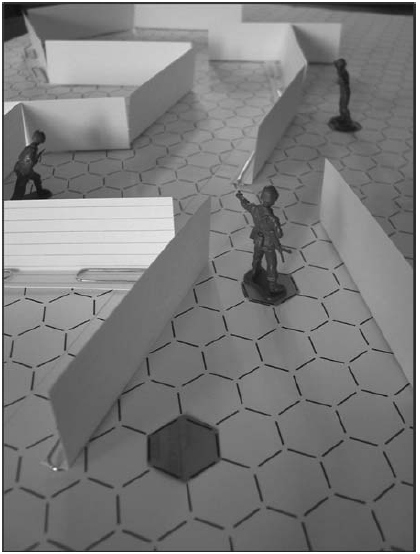
\includegraphics[scale=0.55]{./img/fps-fisical-prototype.png}
 %% matrixargseg.png: 296x162 pixel, 100dpi, 7.52x4.11 cm, bb=0 0 213 117
 %%\caption{Estágio desenvolvimento de jogos ~\cite{fullerton2008game}}
%\caption{Prototipação Física de um \ac{fps} ~\cite{fullerton2008game}}
%%  \caption{Estágio desenvolvimento de jogos}
 %\label{fig:proto-fps}
%\end{figure}

%Uma das etapas do planejamento do designer passa pela concretização da suas ideias através de modelos que consigam certificar de que a concepção é realmente divertida e através de protótipos será possível demonstrá-la para os demais membros da equipe, garantindo que será dada continuidade ao projeto para a produção definitiva ~\cite{prototipgames2007}. Os benefícios do uso de protótipos rápidos é que ele permite testes rápidos de componentes separadamente sem necessariamente implementar o sistema completo como também encoraja usuários a comentar livremente e sugerir modificações (contrário a um produto bem acabado que pode parecer já terminado). Porém, como ponto negativo, temos muitas vezes componentes individuais devem ser re-testados no produto finalizado ~\cite{prototipgames2007}.


%
%
%
%
%\subsection{Protótipo Jogável}
%Game prototypes, while playable, usually include only a rough approximation of the artwork, sound, and features. They are very much like sketches whose purpose is to allow you to focus on a small set of the game’s ~\cite{fullerton2008game}. There are many types of prototypes, including physical prototypes, visual prototypes, video prototypes, software prototypes, etc. 
%
%Prototyping lies at the heart of good game design. Prototyping is the creation of a working model of your idea that allows you to test its feasibility and make improvements to it ~\cite{fullerton2008game}. 
%
%%Buskirk e Moroney [2003] afirmam que o uso da técnica de prototipagem pode ser estendido para outras fases do ciclo de vida do produto além dos testes de usabilidade. Sendo usado na validação dos requisitos junto aos consumidores, na fase de especificação do projeto, desenvolvimento dos manuais do produto, suporte ao marketing, execução de testes funcionais, ajuda no serviço de atendimento aos clientes ~\cite{prototipgames2007}.O público-alvo dessa avaliação inicial inclui publishers, engenheiros de software, artistas, e outros membros da equipe. Como “palavras são fundamentalmente uma maneira terrível de comunicar interatividade” [Waugh 2006], podemos tomar o desenvolvimento de protótipos como meio para ajudar a educar a equipe de como alguns componentes do jogo deveriam se comportar, esclarecendo de forma mais amigável os conceitos abstratos e poder transmitir como o jogo deve funcionar ~\cite{prototipgames2007}.
%If you try to design the entire game at once, you might become confused and overwhelmed. There are so many elements in a typical game that it is diffi cult to know where and how to start. What we recommend is that you isolate the core gameplay mechanisms and build out from there ~\cite{fullerton2008game}.
%
%
%
%\subsection{GAHME Actions Guideline}\label{subsec:game_actions_guide}
%
%Para elaboração deste artefato o \textit{Game Health Designer}, utilizará como irá utilizar as Diretrizes Médicas como base científica de conhecimento e das especificações dos sensores de captura que poderão ser utilizados.
%
%Para elaboração deste artefato o 
%
%Para a sua elaboração o responsável Os artefatos de entrada para elaboração
%
%O responsável pela elaboração do GAHME Actions Design é o que deverá se basear nas Diretrizes Médicas, para fazer uma avaliação dos mPara elaboração do GAHME Actions Design, o autor 
%
%Nesse artefato é levado em consideração o sensor utilizado, o sintoma a ser monitorado e a eficácia do monitoramento sendo comprovada por intermédio de testes efetuados na atividade \textit{Testar Protótipos} da fase de \textit{Prototipação}.
%
%The core gameplay mechanism, or “coremechanic,” can be defi ned as the actions that a player repeats most o en while striving to achieve the game’s overall goal. Games are repetitive by nature. While the meaning and consequences of what a player does can change over the course of game, the core actions tend to remain the same from beginning to end ~\cite{fullerton2008game}.
%
%Creating a physical prototype is a critical step in the design of your original game concept. It will save your team tremendous amounts of time because everyone will have a clear understanding of the game you are making. In addition, a physical prototype will enable you to focus your creative energy on the game mechanics without becoming distracted by the production and programming process ~\cite{fullerton2008game}. 
%
%
%
%\subsection{GAHME Actions Design}
%O objetivo deste artefato é definir quais são os movimentos efetuados pelo jogador dentro do jogo que são passíveis de monitoramento. Para elaboração deste artefato o \textit{GAHME Designer}, irá utilizar as Diretrizes Médicas como base científica de conhecimento e das especificações dos sensores de captura que poderão ser utilizados.
%
%Por promover atividades físicas, ou ações que possam trazer injúria ao jogador, como movimentos de equilíbrio, movimentos repetitivos ou rápidos. O game design do jogo deve ter a preocupação de desenvolver o jogo de acordo com o público-alvo. Isso significa dizer que a faixa etária e limitações físicas e cognitivas em decorrência da idade ou enfermidade devem ser levadas em consideração. Os jogadores devem ter a segurança de usarem o jogo e ter a certeza que o seu uso não acarretará em injúria ~\cite{arntzen2011}.
%
%
%
%
%
%Para elaboração deste artefato o 
%
%Para a sua elaboração o responsável Os artefatos de entrada para elaboração
%
%O responsável pela elaboração do GAHME Actions Design é o que deverá se basear nas Diretrizes Médicas, para fazer uma avaliação dos mPara elaboração do GAHME Actions Design, o autor 
%
%Nesse artefato é levado em consideração o sensor utilizado, o sintoma a ser monitorado e a eficácia do monitoramento sendo comprovada por intermédio de testes efetuados na atividade \textit{Testar Protótipos} da fase de \textit{Prototipação}.
%

